\chapter{Los cinco sentidos}\label{ch:g1:the-five-senses}

Cierra los \omterm{def:g1:the-five-senses:sense}{ojos} y el mundo no desaparece: sigues oyendo la clase,
oliendo la comida que se hace, notando la silla debajo de ti. El
cuerpo tiene cinco puertas al mundo --- los sentidos --- y cada
puerta es un órgano del cuerpo que trabaja para ti todo el día.

\section{Cinco sentidos, cinco órganos}

\begin{definition}[Sentido y órgano de los sentidos]\label{def:g1:the-five-senses:sense}
Un \emph{sentido}\index{sentido} es una manera que tiene el cuerpo de
enterarse de cómo es el mundo. Cada sentido funciona con un
\emph{órgano de los sentidos}\index{órgano de los sentidos}, una parte
del cuerpo hecha para esa tarea:
\begin{enumerate}
  \item la \emph{vista}\index{vista} --- los \emph{ojos}\index{ojo}
        ven la luz, los colores y las formas;
  \item el \emph{oído}\index{oído} --- las \emph{orejas}\index{oreja}
        oyen los sonidos;
  \item el \emph{olfato}\index{olfato} --- la \emph{nariz}\index{nariz}
        huele los olores;
  \item el \emph{gusto}\index{gusto} --- la \emph{lengua}\index{lengua}
        saborea la comida;
  \item el \emph{tacto}\index{tacto} --- la \emph{piel}\index{piel},
        por todo el cuerpo, nota lo áspero y lo suave, lo caliente y lo frío.
\end{enumerate}
\end{definition}

\begin{example}[El desayuno, sentido a sentido]\label{ex:g1:the-five-senses:breakfast}
Un tazón de chocolate caliente usa los cinco: los \omterm{def:g1:the-five-senses:sense}{ojos} ven el vaho,
la nariz huele el cacao, la \omterm{def:g1:the-five-senses:sense}{piel} de las manos nota el tazón caliente,
las \omterm{def:g1:the-five-senses:sense}{orejas} oyen tintinear la cuchara y la lengua --- la mejor parte
--- lo saborea.
\end{example}

\begin{omfigure}
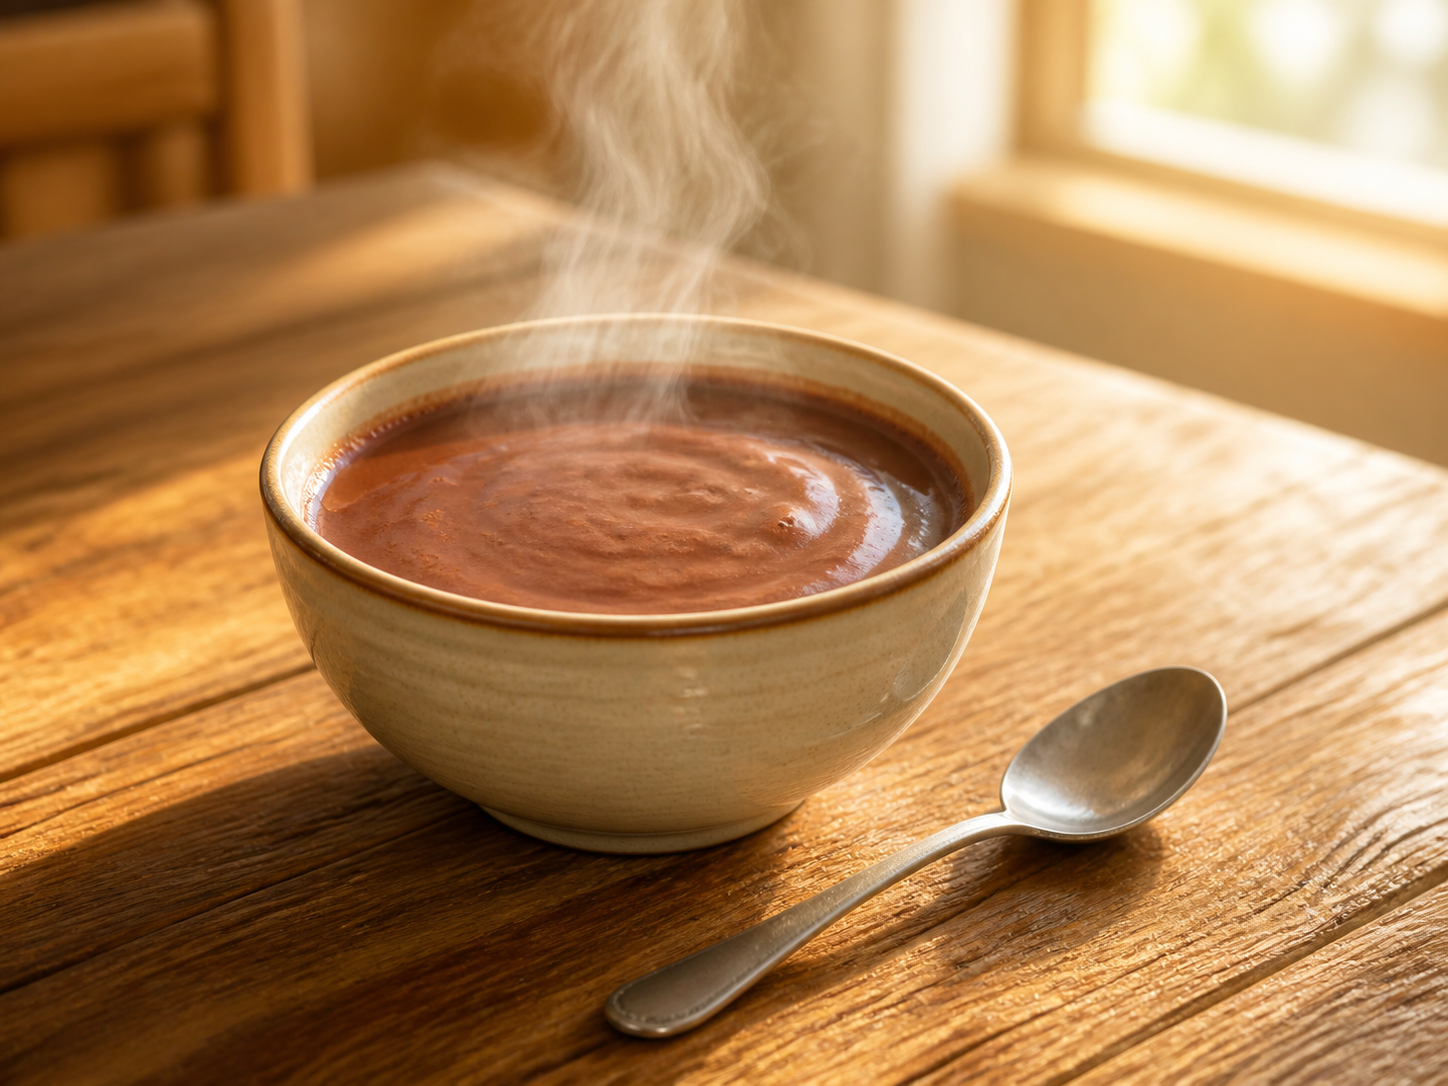
\includegraphics[width=0.58\linewidth]{images/book1/ai/g1-senses-chocolate.png}

{\small Un tazón de chocolate caliente, cinco sentidos trabajando
antes del primer sorbo.}
\end{omfigure}

\begin{remark}[El tacto está por todas partes]\label{rem:g1:the-five-senses:skin}
Cuatro \omterm{def:g1:the-five-senses:sense}{órganos de los sentidos} viven en la cabeza, pero el órgano del
tacto es la \omterm{def:g1:the-five-senses:sense}{piel}, y la \omterm{def:g1:the-five-senses:sense}{piel} te cubre de la cabeza a los pies. Por eso
notas una brisa en el cuello, un guijarro en el zapato y una mariquita
que se posa en tu \omterm{def:g1:my-body:parts}{brazo} --- todo sin mirar.
\end{remark}

\section{Los sentidos avisan al cerebro}

\begin{proposition}[Mensajes al cerebro]\label{prop:g1:the-five-senses:brain}
Un \omterm{def:g1:the-five-senses:sense}{órgano de los sentidos} no entiende lo que capta --- \emph{envía un
mensaje}. Todos los mensajes viajan por dentro del cuerpo hasta el
\emph{cerebro}\index{cerebro}, en la cabeza, que los junta: ``esa es
la voz de la abuela'', ``ese olor es de tostada''. Sin el cerebro, los
\omterm{def:g1:the-five-senses:sense}{ojos} y las \omterm{def:g1:the-five-senses:sense}{orejas} no informarían a nadie.
\end{proposition}
\admitted

\begin{omfigure}
\begin{tikzpicture}[scale=0.9]
  % brain box
  \draw[thick, omDef, fill=omDef!8, rounded corners=6pt]
    (4.6,0.2) rectangle (8.2,2.0);
  \node[font=\small\bfseries, omDef] at (6.4,1.55) {el cerebro};
  \node[font=\small, align=center, text width=3.2cm] at (6.4,0.85)
    {junta los\\ mensajes};
  % organs
  \node[font=\small, left] (eye) at (2.2,2.6) {el ojo ve};
  \node[font=\small, left] (ear) at (2.2,1.7) {la oreja oye};
  \node[font=\small, left] (nose) at (2.2,0.8) {la nariz huele};
  \node[font=\small, left] (skin) at (2.2,-0.1) {la piel nota};
  % arrows
  \draw[->, thick, omMeth] (2.35,2.55) -- (4.55,1.75);
  \draw[->, thick, omMeth] (2.35,1.68) -- (4.55,1.35);
  \draw[->, thick, omMeth] (2.35,0.82) -- (4.55,0.95);
  \draw[->, thick, omMeth] (2.35,-0.02) -- (4.55,0.55);
  \node[font=\small, omMeth] at (3.4,3.0) {mensajes};
\end{tikzpicture}

{\small Cada \omterm{def:g1:the-five-senses:sense}{órgano de los sentidos} envía su mensaje al cerebro, que
les encuentra sentido a todos. (La lengua también informa --- el
dibujo se quedaría sin sitio.)}
\end{omfigure}

\begin{example}[Nombrar cosas a oscuras]\label{ex:g1:the-five-senses:dark}
Un amigo te pone en las manos un objeto conocido con los \omterm{def:g1:the-five-senses:sense}{ojos}
cerrados: una llave, una esponja, una cuchara. Lo nombras casi al
instante. La \omterm{def:g1:the-five-senses:sense}{piel} envió su mensaje --- frío, duro, con picos --- y el
cerebro respondió: ``una llave''. Los sentidos recogen; el cerebro
entiende.
\end{example}

\begin{remark}[Ayudarse unos a otros]\label{rem:g1:the-five-senses:together}
Los sentidos trabajan en equipo. La comida ``sabe'' sosa cuando un
resfriado te tapa la nariz, porque el olfato hacía la mitad del
trabajo del sabor. Y cuando un sentido no puede hacer su tarea, los
demás aprenden a hacer más: las personas que no ven leen con las
yemas de los dedos, con el tacto, y cruzan la calle con las \omterm{def:g1:the-five-senses:sense}{orejas}.
\end{remark}

\section{Cuidar los órganos de los sentidos}

\begin{proposition}[Puertas frágiles]\label{prop:g1:the-five-senses:fragile}
Los \omterm{def:g1:the-five-senses:sense}{órganos de los sentidos} son valiosos y fáciles de estropear. Un
sonido demasiado fuerte daña las \omterm{def:g1:the-five-senses:sense}{orejas}; mirar al Sol daña los \omterm{def:g1:the-five-senses:sense}{ojos};
una cucharada demasiado caliente quema la lengua. Un \omterm{def:g1:the-five-senses:sense}{órgano de los
sentidos} dañado puede quedarse así --- por eso los protegemos.
\end{proposition}
\admitted

\begin{method}[Proteger mis sentidos]\label{met:g1:the-five-senses:protect}
\begin{enumerate}
  \item no mires nunca al Sol de frente, ni un instante;
  \item mantén los sonidos suaves: nada de gritar en las \omterm{def:g1:the-five-senses:sense}{orejas},
        auriculares a poco volumen;
  \item no te metas nunca nada en la \omterm{def:g1:the-five-senses:sense}{oreja} ni en la nariz;
  \item sopla la comida caliente antes de probarla;
  \item lee y dibuja con buena luz.
\end{enumerate}
\end{method}

\begin{example}[El concierto de al lado]\label{ex:g1:the-five-senses:loud}
Después de música muy fuerte, a veces las \omterm{def:g1:the-five-senses:sense}{orejas} pitan un rato. Ese
pitido es la \omterm{def:g1:the-five-senses:sense}{oreja} diciendo ``¡demasiado!''. Quien trabaja con
máquinas ruidosas lleva orejeras justo por eso --- sus oídos tienen
que durarle toda la vida.
\end{example}

\section{Ejercicios}

\begin{exercise}[$\star$]\label{exo:g1:the-five-senses:1}
Nombra los cinco sentidos y, de cada uno, su \omterm{def:g1:the-five-senses:sense}{órgano de los sentidos}.
\end{exercise}

\begin{exercise}[$\star$]\label{exo:g1:the-five-senses:2}
¿Qué \omterm{def:g1:the-five-senses:sense}{órgano de los sentidos} informa: (a) del color de un globo? (b) de
lo suave que es una manta? (c) del olor a lluvia? (d) del sonido de
una campana?
\end{exercise}

\begin{exercise}[$\star$]\label{exo:g1:the-five-senses:3}
¿Qué \omterm{def:g1:the-five-senses:sense}{órgano de los sentidos} no está en la cabeza? ¿Hasta dónde llega?
\end{exercise}

\begin{exercise}[$\star$]\label{exo:g1:the-five-senses:4}
En el \cref{ex:g1:the-five-senses:dark} los \omterm{def:g1:the-five-senses:sense}{ojos} estaban cerrados.
¿Qué órgano envió el mensaje y qué parte del cuerpo lo entendió?
\end{exercise}

\begin{exercise}[$\star$]\label{exo:g1:the-five-senses:5}
Con un resfriado y la nariz tapada, la comida parece perder su sabor.
¿Qué dos sentidos suelen hacer equipo cuando comes?
\end{exercise}

\begin{exercise}[$\star$]\label{exo:g1:the-five-senses:6}
Da tres reglas del \cref{met:g1:the-five-senses:protect} y di qué
\omterm{def:g1:the-five-senses:sense}{órgano de los sentidos} protege cada una.
\end{exercise}

\begin{exercise}[$\star$]\label{exo:g1:the-five-senses:7}
¿Por qué llevan orejeras las personas que trabajan con máquinas
ruidosas? Usa la \cref{prop:g1:the-five-senses:fragile}.
\end{exercise}

\begin{exercise}[$\star$]\label{exo:g1:the-five-senses:8}
Pruébalo: con los \omterm{def:g1:the-five-senses:sense}{ojos} cerrados, deja que alguien te ponga tres
alimentos bajo la nariz --- por ejemplo plátano, queso y naranja.
¿Cuántos acertó tu nariz sin la ayuda de los \omterm{def:g1:the-five-senses:sense}{ojos}?
\end{exercise}

\begin{exercise}[$\star\star$]\label{exo:g1:the-five-senses:9}
Un amigo afirma: ``El \omterm{def:g1:the-five-senses:sense}{ojo} entiende lo que ve''. Corrige la frase con
la \cref{prop:g1:the-five-senses:brain}: ¿qué hace de verdad el \omterm{def:g1:the-five-senses:sense}{ojo} y
quién es el que entiende?
\end{exercise}

\begin{exercise}[$\star\star$]\label{exo:g1:the-five-senses:10}
¿Cómo puede una persona que no ve ``leer'' un libro y cruzar la calle
sin peligro? Di qué sentidos se hacen cargo de qué tareas.
\end{exercise}
